\documentclass{article}
% Use the TikZ bounding box as the PDF page size (pdfLaTeX).
\usepackage{tikz}
\newsavebox{\plotbox}
\newcommand{\startplot}{\begin{lrbox}{\plotbox}\ignorespaces}
\newcommand{\finishplot}{\unskip\end{lrbox}%
  \pdfhorigin=2pt\pdfvorigin=2pt
  \pdfpagewidth=\dimexpr\wd\plotbox+4pt\relax
  \pdfpageheight=\dimexpr\ht\plotbox+\dp\plotbox+4pt\relax
  \shipout\box\plotbox}

\usetikzlibrary{arrows.meta}
\definecolor{ink}{HTML}{203A3C}
\definecolor{sub}{HTML}{445957}
\definecolor{axis}{HTML}{81938B}
\definecolor{acc}{HTML}{965236}
\definecolor{c0}{HTML}{9A563B}
\definecolor{f0}{HTML}{F6EBE0}
\definecolor{c1}{HTML}{7B736A}
\definecolor{f1}{HTML}{F6F0E8}
\definecolor{c2}{HTML}{627A77}
\definecolor{f2}{HTML}{EDF0E8}
\definecolor{c3}{HTML}{497878}
\definecolor{f3}{HTML}{E2ECE8}
\definecolor{c4}{HTML}{246368}
\definecolor{f4}{HTML}{D1E6DF}
\begin{document}\startplot
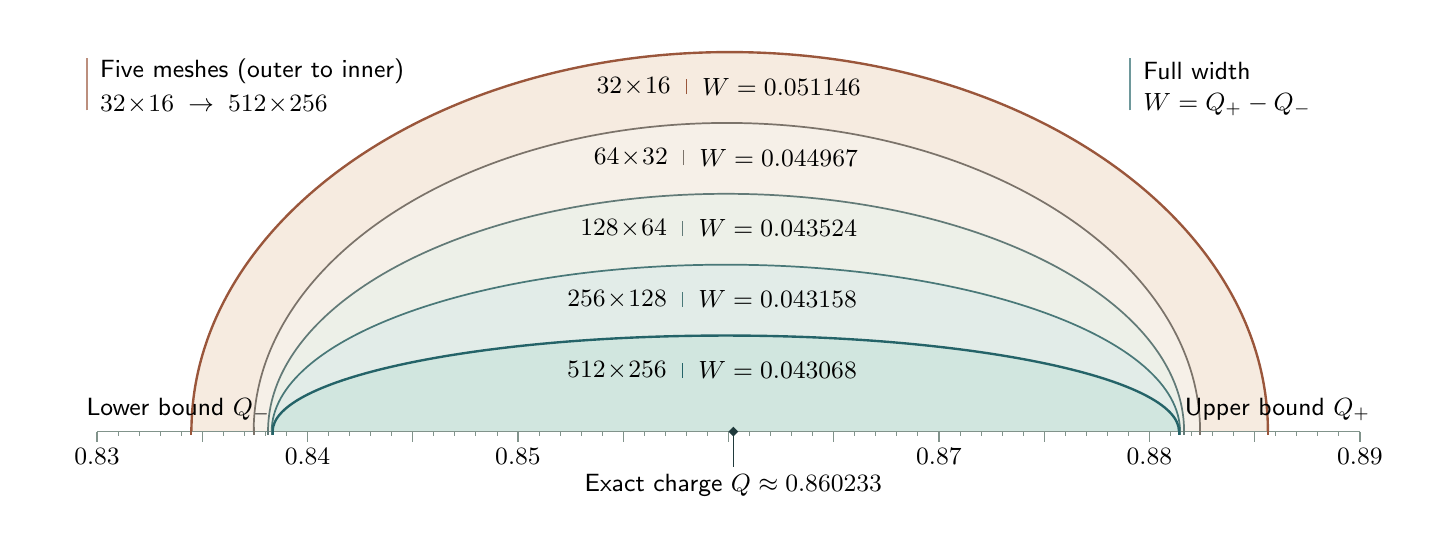
\begin{tikzpicture}[x=1cm,y=1cm,inner sep=0pt,outer sep=0pt,text=black]
\path[use as bounding box] (0,0) rectangle (17.77,6.25);
\path[fill=f0] (2.079609,1.120000) arc[start angle=180,end angle=0,x radius=6.835698cm,y radius=4.820000cm] -- cycle;
\draw[c0,line width=0.86pt] (2.079609,1.120000) arc[start angle=180,end angle=0,x radius=6.835698cm,y radius=4.820000cm];
\path[fill=f1] (2.869997,1.120000) arc[start angle=180,end angle=0,x radius=6.009880cm,y radius=3.920000cm] -- cycle;
\draw[c1,line width=0.62pt] (2.869997,1.120000) arc[start angle=180,end angle=0,x radius=6.009880cm,y radius=3.920000cm];
\path[fill=f2] (3.052493,1.120000) arc[start angle=180,end angle=0,x radius=5.817050cm,y radius=3.020000cm] -- cycle;
\draw[c2,line width=0.62pt] (3.052493,1.120000) arc[start angle=180,end angle=0,x radius=5.817050cm,y radius=3.020000cm];
\path[fill=f3] (3.098818,1.120000) arc[start angle=180,end angle=0,x radius=5.768142cm,y radius=2.120000cm] -- cycle;
\draw[c3,line width=0.62pt] (3.098818,1.120000) arc[start angle=180,end angle=0,x radius=5.768142cm,y radius=2.120000cm];
\path[fill=f4] (3.110248,1.120000) arc[start angle=180,end angle=0,x radius=5.756115cm,y radius=1.220000cm] -- cycle;
\draw[c4,line width=0.86pt] (3.110248,1.120000) arc[start angle=180,end angle=0,x radius=5.756115cm,y radius=1.220000cm];
\node[font=\sffamily\small,text=black,anchor=east] at (8.16531,5.50000) {$32\!\times\!16$};
\draw[c0,line width=.42pt] (8.36531,5.40500) -- (8.36531,5.59500);
\node[font=\sffamily\small,text=black,anchor=west] at (8.56531,5.50000) {$W=0.051146$};
\node[font=\sffamily\small,text=black,anchor=east] at (8.12988,4.60000) {$64\!\times\!32$};
\draw[c1,line width=.42pt] (8.32988,4.50500) -- (8.32988,4.69500);
\node[font=\sffamily\small,text=black,anchor=west] at (8.52988,4.60000) {$W=0.044967$};
\node[font=\sffamily\small,text=black,anchor=east] at (8.11954,3.70000) {$128\!\times\!64$};
\draw[c2,line width=.42pt] (8.31954,3.60500) -- (8.31954,3.79500);
\node[font=\sffamily\small,text=black,anchor=west] at (8.51954,3.70000) {$W=0.043524$};
\node[font=\sffamily\small,text=black,anchor=east] at (8.11696,2.80000) {$256\!\times\!128$};
\draw[c3,line width=.42pt] (8.31696,2.70500) -- (8.31696,2.89500);
\node[font=\sffamily\small,text=black,anchor=west] at (8.51696,2.80000) {$W=0.043158$};
\node[font=\sffamily\small,text=black,anchor=east] at (8.11636,1.90000) {$512\!\times\!256$};
\draw[c4,line width=.42pt] (8.31636,1.80500) -- (8.31636,1.99500);
\node[font=\sffamily\small,text=black,anchor=west] at (8.51636,1.90000) {$W=0.043068$};
\draw[axis,line width=.57pt] (0.88095,1.12000) -- (16.91905,1.12000);
\draw[axis,line width=.48pt] (0.88095,1.12000) -- (0.88095,0.99000);
\node[anchor=north,text=black,font=\small] at (0.88095,0.90000) {0.83};
\draw[axis,line width=.29pt] (1.14825,1.12000) -- (1.14825,1.06000);
\draw[axis,line width=.29pt] (1.41556,1.12000) -- (1.41556,1.06000);
\draw[axis,line width=.29pt] (1.68286,1.12000) -- (1.68286,1.06000);
\draw[axis,line width=.29pt] (1.95016,1.12000) -- (1.95016,1.06000);
\draw[axis,line width=.48pt] (2.21746,1.12000) -- (2.21746,0.99000);
\draw[axis,line width=.29pt] (2.48476,1.12000) -- (2.48476,1.06000);
\draw[axis,line width=.29pt] (2.75206,1.12000) -- (2.75206,1.06000);
\draw[axis,line width=.29pt] (3.01937,1.12000) -- (3.01937,1.06000);
\draw[axis,line width=.29pt] (3.28667,1.12000) -- (3.28667,1.06000);
\draw[axis,line width=.48pt] (3.55397,1.12000) -- (3.55397,0.99000);
\node[anchor=north,text=black,font=\small] at (3.55397,0.90000) {0.84};
\draw[axis,line width=.29pt] (3.82127,1.12000) -- (3.82127,1.06000);
\draw[axis,line width=.29pt] (4.08857,1.12000) -- (4.08857,1.06000);
\draw[axis,line width=.29pt] (4.35587,1.12000) -- (4.35587,1.06000);
\draw[axis,line width=.29pt] (4.62317,1.12000) -- (4.62317,1.06000);
\draw[axis,line width=.48pt] (4.89048,1.12000) -- (4.89048,0.99000);
\draw[axis,line width=.29pt] (5.15778,1.12000) -- (5.15778,1.06000);
\draw[axis,line width=.29pt] (5.42508,1.12000) -- (5.42508,1.06000);
\draw[axis,line width=.29pt] (5.69238,1.12000) -- (5.69238,1.06000);
\draw[axis,line width=.29pt] (5.95968,1.12000) -- (5.95968,1.06000);
\draw[axis,line width=.48pt] (6.22698,1.12000) -- (6.22698,0.99000);
\node[anchor=north,text=black,font=\small] at (6.22698,0.90000) {0.85};
\draw[axis,line width=.29pt] (6.49429,1.12000) -- (6.49429,1.06000);
\draw[axis,line width=.29pt] (6.76159,1.12000) -- (6.76159,1.06000);
\draw[axis,line width=.29pt] (7.02889,1.12000) -- (7.02889,1.06000);
\draw[axis,line width=.29pt] (7.29619,1.12000) -- (7.29619,1.06000);
\draw[axis,line width=.48pt] (7.56349,1.12000) -- (7.56349,0.99000);
\draw[axis,line width=.29pt] (7.83079,1.12000) -- (7.83079,1.06000);
\draw[axis,line width=.29pt] (8.09810,1.12000) -- (8.09810,1.06000);
\draw[axis,line width=.29pt] (8.36540,1.12000) -- (8.36540,1.06000);
\draw[axis,line width=.29pt] (8.63270,1.12000) -- (8.63270,1.06000);
\draw[axis,line width=.48pt] (8.90000,1.12000) -- (8.90000,0.99000);
\draw[axis,line width=.29pt] (9.16730,1.12000) -- (9.16730,1.06000);
\draw[axis,line width=.29pt] (9.43460,1.12000) -- (9.43460,1.06000);
\draw[axis,line width=.29pt] (9.70190,1.12000) -- (9.70190,1.06000);
\draw[axis,line width=.29pt] (9.96921,1.12000) -- (9.96921,1.06000);
\draw[axis,line width=.48pt] (10.23651,1.12000) -- (10.23651,0.99000);
\draw[axis,line width=.29pt] (10.50381,1.12000) -- (10.50381,1.06000);
\draw[axis,line width=.29pt] (10.77111,1.12000) -- (10.77111,1.06000);
\draw[axis,line width=.29pt] (11.03841,1.12000) -- (11.03841,1.06000);
\draw[axis,line width=.29pt] (11.30571,1.12000) -- (11.30571,1.06000);
\draw[axis,line width=.48pt] (11.57302,1.12000) -- (11.57302,0.99000);
\node[anchor=north,text=black,font=\small] at (11.57302,0.90000) {0.87};
\draw[axis,line width=.29pt] (11.84032,1.12000) -- (11.84032,1.06000);
\draw[axis,line width=.29pt] (12.10762,1.12000) -- (12.10762,1.06000);
\draw[axis,line width=.29pt] (12.37492,1.12000) -- (12.37492,1.06000);
\draw[axis,line width=.29pt] (12.64222,1.12000) -- (12.64222,1.06000);
\draw[axis,line width=.48pt] (12.90952,1.12000) -- (12.90952,0.99000);
\draw[axis,line width=.29pt] (13.17683,1.12000) -- (13.17683,1.06000);
\draw[axis,line width=.29pt] (13.44413,1.12000) -- (13.44413,1.06000);
\draw[axis,line width=.29pt] (13.71143,1.12000) -- (13.71143,1.06000);
\draw[axis,line width=.29pt] (13.97873,1.12000) -- (13.97873,1.06000);
\draw[axis,line width=.48pt] (14.24603,1.12000) -- (14.24603,0.99000);
\node[anchor=north,text=black,font=\small] at (14.24603,0.90000) {0.88};
\draw[axis,line width=.29pt] (14.51333,1.12000) -- (14.51333,1.06000);
\draw[axis,line width=.29pt] (14.78063,1.12000) -- (14.78063,1.06000);
\draw[axis,line width=.29pt] (15.04794,1.12000) -- (15.04794,1.06000);
\draw[axis,line width=.29pt] (15.31524,1.12000) -- (15.31524,1.06000);
\draw[axis,line width=.48pt] (15.58254,1.12000) -- (15.58254,0.99000);
\draw[axis,line width=.29pt] (15.84984,1.12000) -- (15.84984,1.06000);
\draw[axis,line width=.29pt] (16.11714,1.12000) -- (16.11714,1.06000);
\draw[axis,line width=.29pt] (16.38444,1.12000) -- (16.38444,1.06000);
\draw[axis,line width=.29pt] (16.65175,1.12000) -- (16.65175,1.06000);
\draw[axis,line width=.48pt] (16.91905,1.12000) -- (16.91905,0.99000);
\node[anchor=north,text=black,font=\small] at (16.91905,0.90000) {0.89};
\draw[c0,line width=.7pt] (2.07961,1.17700) -- (2.07961,1.08000);
\draw[c0,line width=.7pt] (15.75100,1.17700) -- (15.75100,1.08000);
\draw[c1,line width=.7pt] (2.87000,1.17700) -- (2.87000,1.08000);
\draw[c1,line width=.7pt] (14.88976,1.17700) -- (14.88976,1.08000);
\draw[c2,line width=.7pt] (3.05249,1.17700) -- (3.05249,1.08000);
\draw[c2,line width=.7pt] (14.68659,1.17700) -- (14.68659,1.08000);
\draw[c3,line width=.7pt] (3.09882,1.17700) -- (3.09882,1.08000);
\draw[c3,line width=.7pt] (14.63510,1.17700) -- (14.63510,1.08000);
\draw[c4,line width=.7pt] (3.11025,1.17700) -- (3.11025,1.08000);
\draw[c4,line width=.7pt] (14.62248,1.17700) -- (14.62248,1.08000);
\node[anchor=west,font=\sffamily\small,text=black] at (0.74730,1.40000) {Lower bound $Q_-$};
\node[anchor=east,font=\sffamily\small,text=black] at (17.05270,1.40000) {Upper bound $Q_+$};
\draw[ink,line width=.61pt] (8.96215,1.10500) -- (8.96215,0.67000);
\fill[ink] (8.96215,1.12000) ++(0,.062) -- ++(.062,-.062) -- ++(-.062,-.062) -- ++(-.062,.062) -- cycle;
\node[font=\sffamily\small] at (8.96215,0.44000) {Exact charge $Q\approx0.860233$};
\draw[c0!66,line width=.6pt] (0.75000,5.20000) -- (0.75000,5.86000);
\node[anchor=west,font=\sffamily\small,text=black] at (0.92000,5.70000) {Five meshes (outer to inner)};
\node[anchor=west,font=\small,text=black] at (0.92000,5.27000) {\(32\!\times\!16\;\rightarrow\;512\!\times\!256\)};
\draw[c4!66,line width=.6pt] (14.00000,5.20000) -- (14.00000,5.86000);
\node[anchor=west,font=\sffamily\small,text=black] at (14.17000,5.70000) {Full width};
\node[anchor=west,font=\small,text=black] at (14.17000,5.27000) {$W=Q_+-Q_-$};
\end{tikzpicture}
\finishplot\end{document}
